\section{Seating and Mobility Aids}

Seating and mobility aids cover a broad spectrum of assistive technologies such as wheelchairs, scooters, walkers, canes, and crutches. These technologies aim to enhance the mobility and in turn quality of life of the user by helping the control of head, arms and hands, ensuring an improved body stability for ease of movement. Further advanced seating and mobility applications make use of sensors attachable to the assistive technologies that improve the effectiveness of these tools. Some of the most popular applications are smart chair, smart walker/cane, and smart bed. While the target population for these applications is mostly the people with physical impairments and seniors, applications such as the smart bed would also help analyze able-bodied individuals' behavior to avoid possible future health problems \citep{laurino_smart_2020,su_monitoring_2019}. The common characteristic of these applications is that they are equipped with sensors that collect the physiological data both from the user and the environment to monitor and control the user's surroundings. \\

\subsection{Smart Chair}

People with severe physical disabilities are highly dependent on their powered mobility means to go from point A to point B either within their home environment or outside. Not unlike the automotive industry, in the past decade, wheelchair technologies have been advanced, and now evolving from the power wheelchairs (PWs) to smart wheelchairs (SWs) \parencite{leaman_comprehensive_2017}. Traditional PWs require the users to navigate the wheelchair using a hand-rim or a joystick, which may not be accessible by severely disabled users. SWs equipped with advanced assistive technologies, such as human-computer interfaces, sensor arrays, sensor processing algorithms, and machine-vision, have been developed to provide mobility and improved living conditions to those users. SWs not only advance the control and navigation mechanisms of the wheelchair but also elevate the user comfort level as well as usability and safety of the wheelchair in various environments (e.g. indoors, outdoors, rugged train, sloped curbside, etc.) \parencite{ahmad_screen-printed_2019,hu_smart_2020,tavares_wheelchair_2020}.

%In the literature, 
The general approach for developing SWs is to deploy sensors and data processing units to PWs for collecting and analyzing a much wider range of inputs from the user and the environment \parencite{leaman_comprehensive_2017}. The commonly preferred method for controlling and navigating the wheelchair is haptic feedback, which uses various tactile sensors equipped with force sensors \parencite{hadj-abdelkader_haptic_2012,morere_haptic_2015,poorten_powered_2012,trujillo-leon_tactile_2018}. A haptic handlebar using force-sensing resistor sensors (FSR) is proposed in \textcite{trujillo-leon_tactile_2018}. The tactile sensor-based steering, demonstrated in Figure \ref{fig:smart_chair}.a, aims to assist caregivers in navigating the wheelchair. The handlebar is equipped with a matrix of FSRs; the force applied to the handlebar changes the resistivity of the FSRs. The variation in the resistance is converted to voltage by transimpedance amplifiers. The voltage outputs are then digitized by an analog-to-digital converter (ADC) and sent to a personal computer (PC) via a universal serial bus (USB) connection. The digitized output values coming from the sensor matrix compose a pressure map used to control the motion of the wheelchair. 

Being seated for long hours in a wrong position can cause secondary disuse problems such as pressure sores \parencite{redford_seating_1993}; therefore, monitoring the user's sitting posture is critical. \textcite{sen_wireless_2018} proposes a wearable sensor patch that monitors the contact pressure continuously for pressure ulcer prevention. The sensor patch utilizes FSRs for measuring the contact pressure. In \textcite{tavares_wheelchair_2020}, fiber Bragg grating (FBG) sensors are used to detect higher pressure areas during seating to prevent the development of pressure ulcers in wheelchair users. The system is based on the principle that the reflected Bragg wavelength in an optical fiber changes with the variations in fiber strain caused by the pressure as shown in Figure \ref{fig:smart_chair}.b. In the implementation, six FBGs are embedded into a thermosetting epoxy resin cylinder to maintain the fiber's physical integrity and placed in different points on the wheelchair where pressure is applied the most, such as scapulas, ischiatic zones, and heels. Two other FBGs are inserted in separate optical fibers for temperature monitoring; the purpose of temperature monitoring is to analyze the thermal influence on the pressure values since the reflected Bragg wavelength also shifts with temperature variations. 

\begin{figure}[t!]
    \centering
    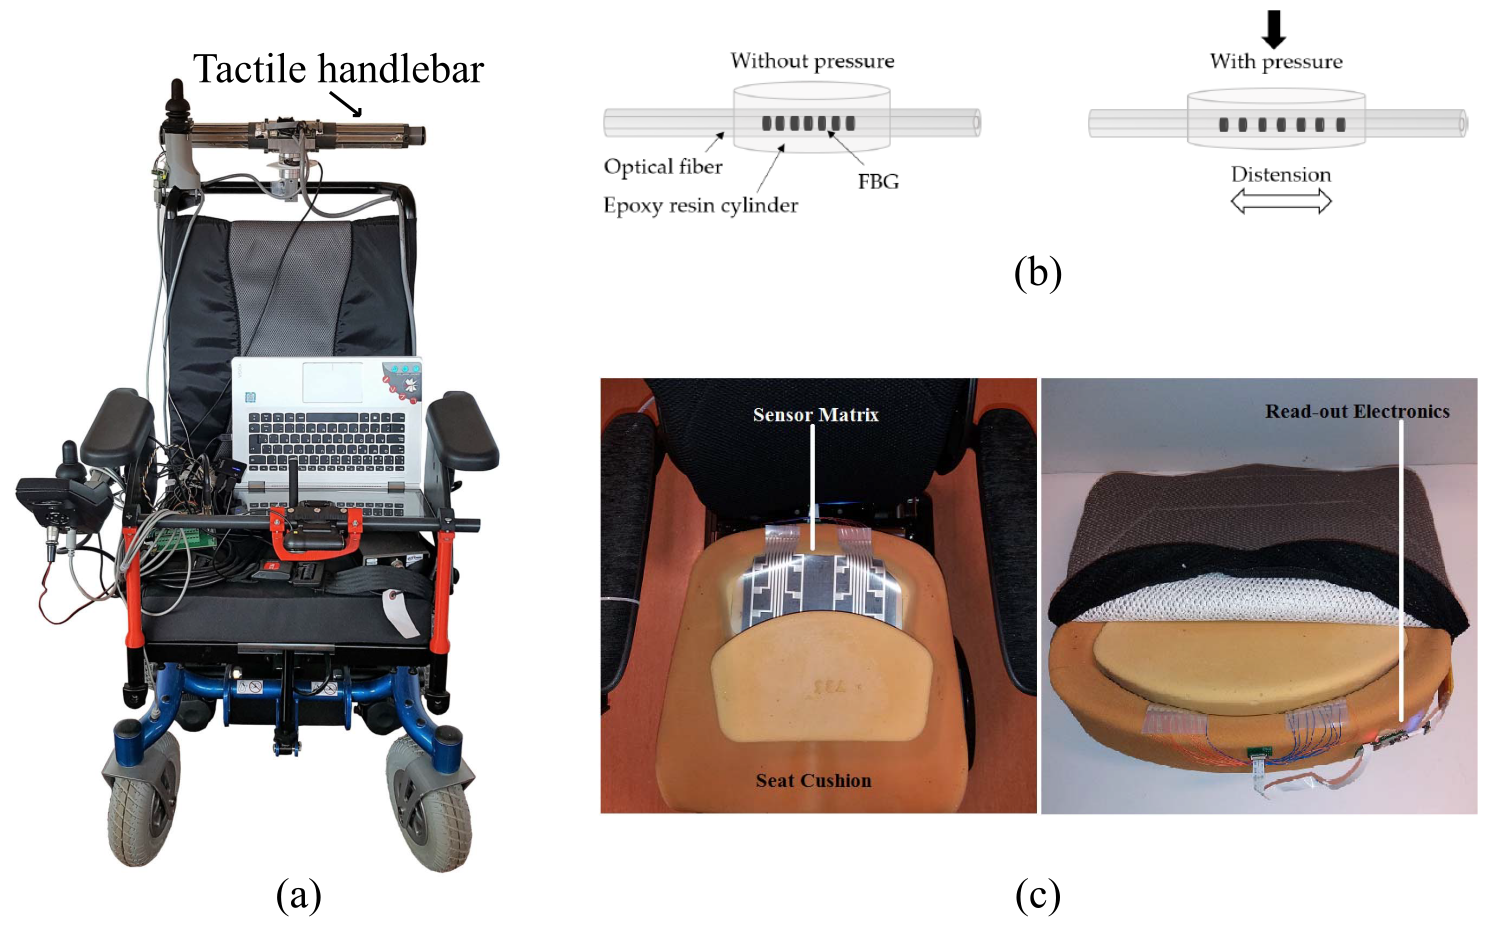
\includegraphics[scale=0.95]{Figure/Seating and Mobility Aids/Smart_chair.PNG}
    \caption{Illustrations from the SW applications. (a)  Setup of the wheelchair with tactile sensor-based steering, modified from \parencite{trujillo-leon_tactile_2018}. (b)  Effect of pressure on the physical structure of the FBG-based pressure sensor, reproduced with permission from \parencite{tavares_wheelchair_2020}.(c) Placement of the pressure sensors in the seat cushion,reproduced with permission from \parencite{ahmad_screen-printed_2019}. }
    \label{fig:smart_chair}
\end{figure}

\textcite{ahmad_screen-printed_2019} presents a screen-printed sensor that measures the pressure distribution on the seat of a wheelchair. The screen-printed sensor consists of 16 piezoresistive sensing elements printed on a polyethylene terephthalate sheet in the form of a $4\times4$ sensor matrix. The sensor matrix is placed underneath the seat cushion, as can be seen in Figure \ref{fig:smart_chair}.c. The data collected from the sensors is sampled using 16 dedicated ADC channels that have a 10-bit resolution. The sampled data is sent to a PC by a Bluetooth module on-board and is processed using MATLAB. \textcite{hu_smart_2020} demonstrates a smart chair design that monitors the user's sitting posture to ensure a healthy seating position by using flex sensors and a field-programmable gate array (FPGA) implemented neural network. The flex sensors, which are sensitive to bending, are placed on an office chair's back and seat. The sensor output is fed into an Arduino microcontroller and a separate ADC module for sampling, outputs of which are given to a PC and an FPGA, respectively. The sampled data received by the PC is used for training the neural network, and the data received by the FPGA is utilized for validation.

\subsection{Smart Walker/Cane} 

%Technology-assisted canes can be equipped with single or multiple sensors depending on the system requirements and operating conditions. 
In the literature, ultrasonic sensors, infrared (IR) sensors, camera, accelerometer, gyroscope, humidity sensor, global positioning system (GPS), which can be considered an outdoors position sensor, are widely employed in the technology-assisted canes \parencite{khan_technology-assisted_2018}. For instance, ultrasonic sensors and cameras are used to detect and recognize objects, while IR sensors are utilized to estimate the distance and stair inclination. The accelerometer detects the steps; the GPS localizes the cane user; the gyroscope detects the cane's orientation \parencite{ahmad_multi-sensor_2018,leal-junior_plane-by-plane_2019,wade_feasibility_2019}.

\textcite{wade_feasibility_2019} presents an instrumented cane system that collects mobility data and assesses the fall risk with the sensors attached to the cane. Force sensing resistors and a 9 degrees of freedom (DOF) inertial measurement unit (IMU) are placed on the cane handle to detect how much grip pressure the user is applying. Afterward, pressure data can be used to figure out potentially harmful usage. The cane's shaft has an RF module that transmits the data from the sensors to a custom dongle and an ultrasound sensor that detects an obstacle. A single-axis load cell is located at the base to measure the weight borne on the cane. A 3DOF accelerometer, also at the base of the cane, is used to measure the linear acceleration. The data collected from the sensors is fed into ADCs, also placed on the cane. Later, the sampled data is sent by the RF module to a PC for processing. 

A standard walker is equipped with load cells and a light detection and ranging (LIDAR) sensor to monitor the walker's usage in \textcite{viegas_monitoring_2018}. The load cells, attached to the walker's base, as shown in Figure \ref{fig:smart_cane}.a,sense the applied force on the walker's legs. The data coming from the cells is analyzed to find the center of mass information. The LIDAR sensor measures the distance traveled by the user and walker. The gathered data is used to monitor the separation between the user and walker, and hence accordingly, the coordination between the walker's movement and the user's gait. The sensor data is collected by a microcontroller and transmitted to a PC, in which an on-board Bluetooth module processes the data. In the data processing part, two risk factors are identified. The first risk factor is based on the balance of forces applied on the walker's legs, and the second one is based on the coordination between the walker's movement and the user's gait. The risk factors are computed using the sensor data. A graphical user interface (GUI) is created to monitor both the sensor data and risk factors in real-time.

\textcite{meshram_astute_2019} proposes a cane that can detect obstacles, familiar objects, and wet floors in the environment to assist visually impaired people. The obstacle detection is achieved by utilizing five ultrasonic sensors on different locations of the cane's shaft. At the top of the cane, the radio-frequency identification (RFID) reader recognizes the objects with an RFID tag in the environment.
% Because of the tag's location, the system cannot identify the unfamiliar (non-tagged) objects, which is a downside of the system that needs to be improved. 
At the base of the cane, a liquid contact sensor detects the wet floors. The placement of the sensors is shown in Figure \ref{fig:smart_cane}.b. The sensor data is processed on a small computer located on the cane's body. After processing the sensor data, the smart cane provides information to the user about the obstacles and objects in the environment through tactile feedback using the vibrator at the cane's handle or auditory feedback using wired/wireless headphones. 

\begin{figure}[h!]
    \centering
    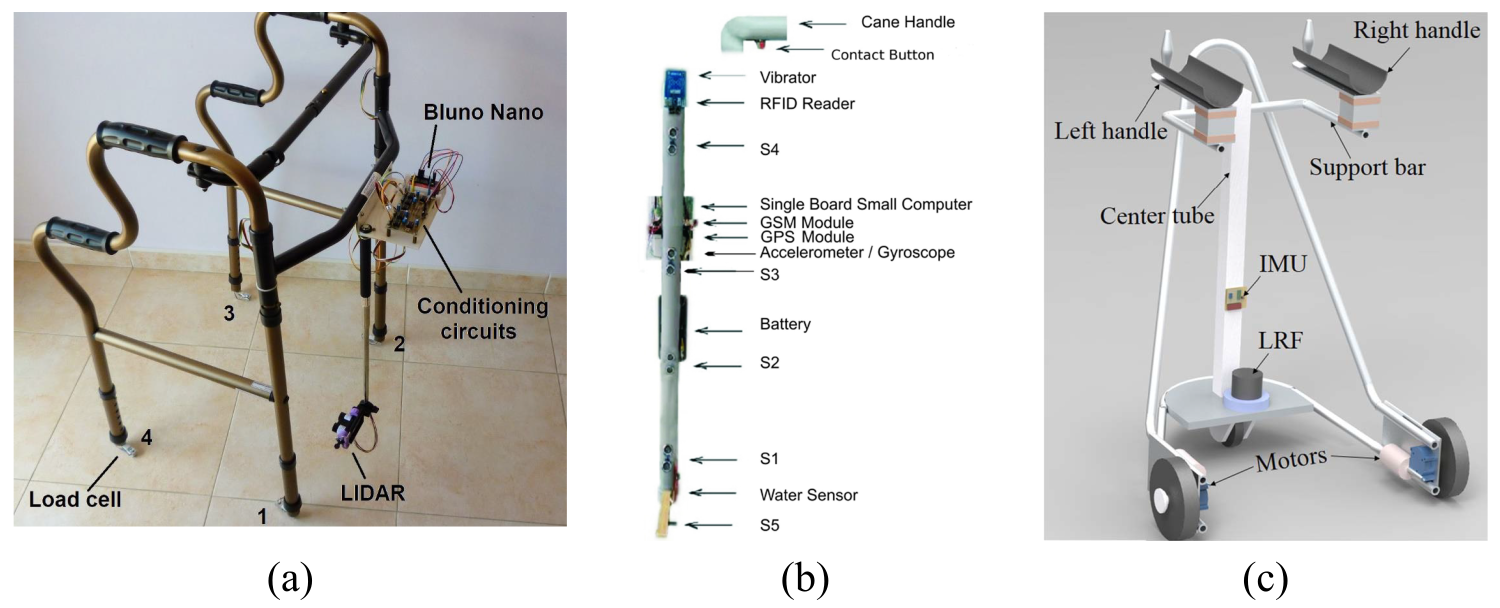
\includegraphics[scale=0.95]{Figure/Seating and Mobility Aids/Smart_cane.PNG}
    \caption{Illustrations of smart walker/cane applications. (a) A standard walker equipped with load cells and a LIDAR to assist the user, from \parencite{viegas_monitoring_2018}, (b)  A cane with various sensors that aims to guide visually impaired people, reproduced with permission from \parencite{meshram_astute_2019}, (c) Overview of the SW used for the fiber Bragg grating (FBG) array implementation, FBG array is placed on the support bar. Reproduced with permission from \parencite{leal-junior_plane-by-plane_2019}.}
    \label{fig:smart_cane}
\end{figure}

A fiber Bragg grating (FBG) based smart walker is presented in \textcite{leal-junior_plane-by-plane_2019}, which can monitor the temperature, strain, and vibrational oscillations to estimate the gait cadence, the floor vibration condition, and the force applied to the walker by the user. The working principle of the FBG sensors is based on the shift of the Bragg wavelength due to temperature variations and strain. Five FBGs are placed on the walker's support bar to capture the force applied by the user and vibrational oscillations due to the floor level variations. In order to evaluate the data obtained by the FBGs, the authors deployed force sensors in the walker's handle, an inertial measurement unit on the walker's shaft, and also a laser range finder at the walker's base, as shown in Figure \ref{fig:smart_cane}.c, to compare force measurements, vibrational oscillations, and gait cadence data, respectively.

\subsection{Smart Bed}

Continuously monitoring the vital sign parameters such as blood pressure, cardiac and respiratory rates is of great importance to detect cardiac and respiratory diseases at an early stage and assess sleep quality. The gold standard for monitoring the vital signs during sleep is the polysomnography method \parencite{jafari_polysomnography_2010}, an obtrusive method, which is not suitable for use in home settings. Hence, the recent research in smart bed applications is focused on unobtrusive methods that can be employed both in a professional setting and a home-care environment \parencite{laurino_smart_2020,su_monitoring_2019,waltisberg_detecting_2017,wang_noninvasive_2020,yu_multi-modal_2019}. 

These applications rely on noninvasive sensor technologies generally placed in the bed mattress. These sensors can create the pressure map of the body, which provides information on respiratory and cardiac rates when continuously generated by utilizing piezoresistive, capacitive, optical, and piezoelectric sensors \parencite{laurino_smart_2020,waltisberg_detecting_2017,wang_noninvasive_2020}; ballistocardiography is another popular method to measure blood pressure and heart rate \parencite{su_monitoring_2019,yu_multi-modal_2019}. There are also applications in which the sensors are located around the smart bed setting to measure respiration; camera sensors, ultrasonic proximity sensors, multi-walled carbon nanotubes sensors are among the frequently used sensor solutions for such applications.

\textcite{laurino_smart_2020} proposed a smart bed with multi-modal sensing for the assessment of sleep quality based on multiple parameters. The data for the assessment is collected from two different sensor interfaces. The first interface collects information from the user's body, and it is called physiological data collector (PDC). The second interface gathers data from the environment, and it is called environmental data collector (EDC). The PDC is equipped with textile pressure arrays (piezoresistive sensors), lied on the bed, as demonstrated in Figure \ref{fig:smart_bed},  and tri-axial accelerometers, also placed on the bed, for monitoring the position, movement, breath, and heart rates of the user. The ability to detect position, movement, breathing and heart rate simultaneously is the key specification of the proposed smart bed, which differentiates it from the other literature that provide single mode solutions. The EDC has sensors that collect sound intensity, temperature, relative humidity, and luminosity data from the environment. The sensor data coming from the EDC and PDC sensors is processed in a docking station. A sleep-quality algorithm generates a global sleep-quality index that  assesses the sleep quality of the user. 

\begin{figure}
    \centering
    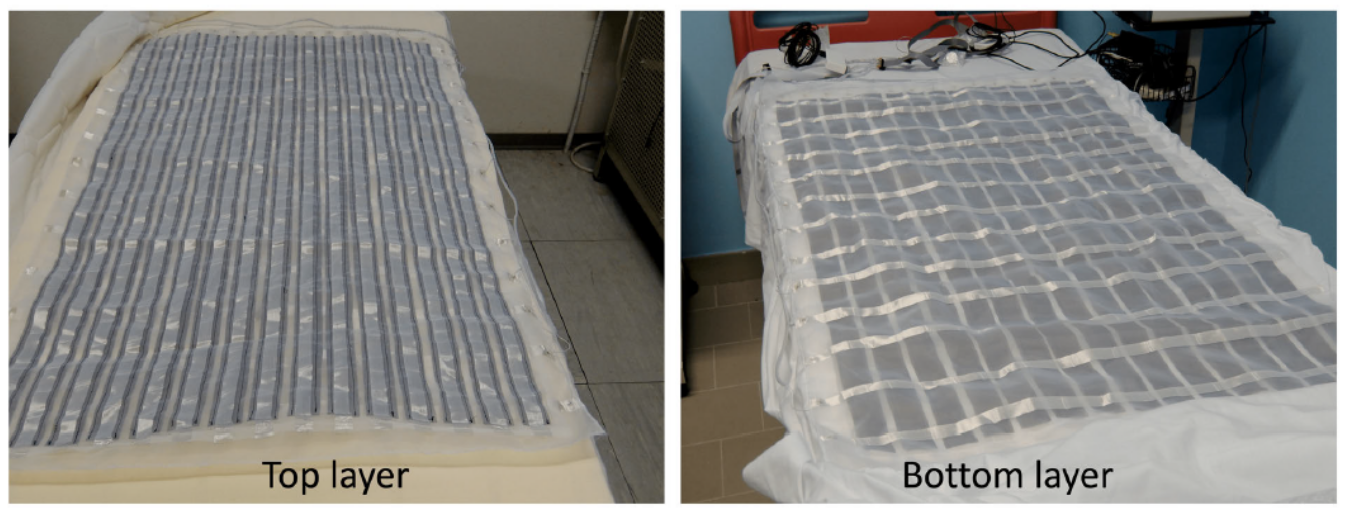
\includegraphics[scale=1]{Figure/Seating and Mobility Aids/Smart_bed.PNG}
    \caption{Textile pressure mapping system based on a textile resistive matrix with 13 column conductors and 15 row conductors for a total of 195 sensing areas, from \parencite{laurino_smart_2020}.}
    \label{fig:smart_bed}
\end{figure}

In another study, an array of strain gauges placed between the bed mattress and the bed frame to sense the pressure variations on the bed mattress to monitor the user's body movements and respiration \parencite{waltisberg_detecting_2017}. The aim of monitoring these body signs is to understand the sleep-related breathing and movement disorders and guide the treatment procedure. The sensor array is composed of eight uniformly distributed strain gauges, and the total size of the array is 72 cm by 16 cm, which covers the whole width of the bed. Two fusion methods were applied in the processing of the sensor data, namely measurement and decision fusion; both methods include filtering, feature extraction, normalization, and classification algorithms. 

\textcite{wang_noninvasive_2020} presents a smart mattress that can be used for household and hospital health monitoring. Optical fiber Mach-Zender interferometer (MZI) senses the pressure variations due to cardiac and breathing activities; sensor outputs are then processed and analyzed to generate information about the user's health status. The optical fiber MZI is composed of a laser source, couplers, single-mode fibers, and photodetectors. In the proposed design, the sensing arm is placed in the mattress, and reference fiber is arranged in a separate terminal box. The optical phase difference between the reference and the sensing fibers is proportional to the signal path length of these fibers. When a pressure is applied on the mattress, the path length of the signal travelling in the sensing fiber changes that varies the phase difference between the reference and sensing fibers. The photodetectors can read the variations of the phase difference at the outputs of the optical fiber MZI. The raw pressure variation data is used to extract the cardiac activity information after passing through several processing steps. 

\textcite{su_monitoring_2019} demonstrates a smart bed system that utilizes hydraulic pressure sensors placed underneath the bed mattress to identify two ballistocardiographic (BCG) measures, namely ballistocardiogram pulse strength (BPS) and ballistocardiogram pulse deviation (BPD). The purpose of identifying these metrics is to monitor the blood pressure, which can be used to signify the risk of cardiovascular disorders at an early stage and prevent them. 

\textcite{yu_multi-modal_2019} presents a multi-modal sensor that is a combination of a capacitive electrocardiogram (cECG) electrode, reflective PPG (rPPG), and magnetic induction (MI) sensor for unobtrusively monitoring the vital parameters of the human body, namely the heart and respiration rates. The cECG uses the same principles of a standard ECG to monitor cardiac activity. However, unlike the standard ECG, cECG does not require direct contact with the human skin and can detect the cardiac signals through the layers of various materials such as clothing. The multi-modal sensor integrates the rPPG and MI sensors into the cECG electrode to enable data fusion. The rPPG and MI sensors measure the heart and the respiration rates and complement the measurement data obtained from the cECG electrode to increase the measurement's reliability.


\subsection{Sensors in Use}

\subsubsection{Pressure Sensors} 

Pressure sensors are the most popular type of sensors used in seating and mobility aids. One can classify the pressure sensors according to the sensing principle employed. In this section, 3 classes of the pressure sensors are discussed namely piezoresistive, fiber-optical, and hydraulic sensors. %Pressure sensors can be classified into 3 groups namely the piezoresistive, fiber-optical, and hydraulic sensors.



Flexible semiconductor materials, which resistivity changes with shape deformation (bending, stretching, and compression), are classified as piezoresistive materials \parencite{morris_chapter_2016}. Piezoresistive materials are widely used for force sensing in seating and mobility aids. \textcite{trujillo-leon_tactile_2018} utilizes rectangular force-sensing resistors (FSRs), which are basically piezoresistive sensors. In this application, FSRs are placed on the handlebar (diameter 42.5 mm, length 120 mm) of the wheelchair to detect the force applied by the user on the handlebar.

Piezoresistive sensors (17 mm x 12 mm x 350$\mu$m) screen-printed on a polyethylene terephthalate substrate measure the pressure distribution on the wheelchair seat \parencite{ahmad_screen-printed_2019}; the sensor is capable of sensing 0.1 - 100 N of force. Force sensing resistors with a sensitivity range of 0.2 - 20 N are attached to the cane handle for measuring the grip pressure in \textcite{wade_feasibility_2019}.\textcite{laurino_smart_2020}  mapped pressure by 195 evenly spaced (separated by 3 cm in the rows and 8 cm in the columns) textile piezoresistive sensors made of CARBOTEX 03-82 fabric. \textcite{hu_smart_2020} uses a piezoresistive sensor, called flex sensor, composed of a  polymer ink with conductive particles and plastic flake for pressure sensing. The sensor is 73.7 mm long, has 64.5 mm width and 0.5 mm thickness.

The reflected Bragg wavelength of the FBGs is a pressure and temperature-dependent parameter \parencite{tavares_wheelchair_2020}. Thus one can detect pressure variations by monitoring the change in the reflected Bragg wavelength with compensating for the temperature changes. The fiber optical sensor in \textcite{tavares_wheelchair_2020} comprises six FBGs placed in an epoxy resin cylinder of 2 cm diameter for monitoring the pressure in six different locations on the wheelchair. \textcite{leal-junior_plane-by-plane_2019} utilizes FBGs with 1.57 \pm 0.15  pm($\mu\epsilon^{-1}$) strain sensitivity for sensing the applied force on the walker handle. Unlike the FBG approach, the system in \textcite{wang_noninvasive_2020} is based on MZI with two fiber arms, namely the reference arm and sensing arm. The pressure applied to the sensing fiber increases the path in which the light travels and creates a phase difference between the reference sensor and the sensing sensor, proportional to the amount of pressure.

Hydraulic sensors transduce pressure to an electrical signal and can be used to monitor the relative blood pressure in a smart bed setting \parencite{su_monitoring_2019}. The commonly used hydraulic sensor type is the strain gauge \parencite{waltisberg_detecting_2017}, which produces a variable electrical signal proportional to sensor's elastic deformation.


\subsubsection{Inertia Sensors}

Accelerometers, load cells, and IMUs are frequently-used inertia sensors. Inertia sensors in seating and mobility applications are utilized for position and movement detection \parencite{laurino_smart_2020,viegas_monitoring_2018,wade_feasibility_2019}.

\subsubsection{Range Sensors}

Range sensors are used for obstacle detection, navigation and path detection in smart chair and walker/cane applications. Ultrasound sensors  \parencite{meshram_astute_2019,wade_feasibility_2019} and LIDAR sensors \parencite{viegas_monitoring_2018} are the two widely used range sensors. 

%%%%%%%%%%%%%%%%%%%%%%%%%%%%%%%%%%%%%%%%%%%%%%%%%%%%%%%%%%%%%%%%%%%%%%%%%%%%%%%%%%%%%%%%%%%
